\documentclass[12pt letterpaper]{article}

\usepackage{fullpage}
\usepackage{graphicx}
\usepackage{amsmath}

\providecommand{\e}[1]{\ensuremath{\times 10^{#1}}}




\title{Double Slit Experiment}
\author{Johnny Minor \\ Partner: Kayla Mitchell}
\date{\today}

\begin{document}

\maketitle

%abstract should have a very brief overiew of the goals and main results of the experiment. 
\begin{abstract}
A revolution began when the peculiarities of the wave nature of light became exposed with Young's double slit experiment. The wave nature of light becomes apparent when two slits that are smaller in width than the wavelength of the light are placed in front of a light source. This leads to diffraction of the light. The diffraction will result in both constructive and destructive interference. This creates an interference pattern once the light has passed through the double slit. We measure the intensity of the light for three different settings: left slit, double slit, and right slit. We can then create a plot of the distance across the viewing plate vs. intensity. This will highlight the wave nature of light. We can then conclude that light exhibits wave like properties when passed through an adequately thin double slit. This is important because it is the beginning of what would later become Quantum Mechanics. 

\end{abstract}

\newpage

\section*{Description of Experiment}

\subsection*{History}

During the $17^{th}$ and $18^{th}$ century a debate was raging amongst physicist. The debate was over the whether light was either a particle, or a wave. Originally Sir Isaac Newton proposed that light was a particle. This was his corpuscular theory of light. Since Newton had so much clout in the scientific community everyone followed his thinking without too much criticism at least for about a hundred years. 

Newton's corpuscular theory persisted until Thomas Young proposed that light was a wave in 1800. Young's idea was met with palpable skepticisms as it went against the revered corpuscular theory. So, Young as a good scientist went about trying to prove empirically that light was in fact a wave, or exhibited a wave-like nature. He created the double slit experiment and presented it in 1803. 

It is important to understand the historical significance of this experiment because it was the beginning of the age of understanding that light exhibits both wave and particle nature. Today this is the so called ``wave-particle duality" of light. 

\subsection*{Experiment}

The purpose of this experiment is to replicate Young's experiment and to analyze the interference pattern. Our setup for this experiment was was in figure \ref{fig:double_slit_setup}. All of this was placed inside a metal box apparatus. This was to shield the detectors from stray light. 

\begin{figure}[!ht]
  \caption{The double slit setup}
  \centering
    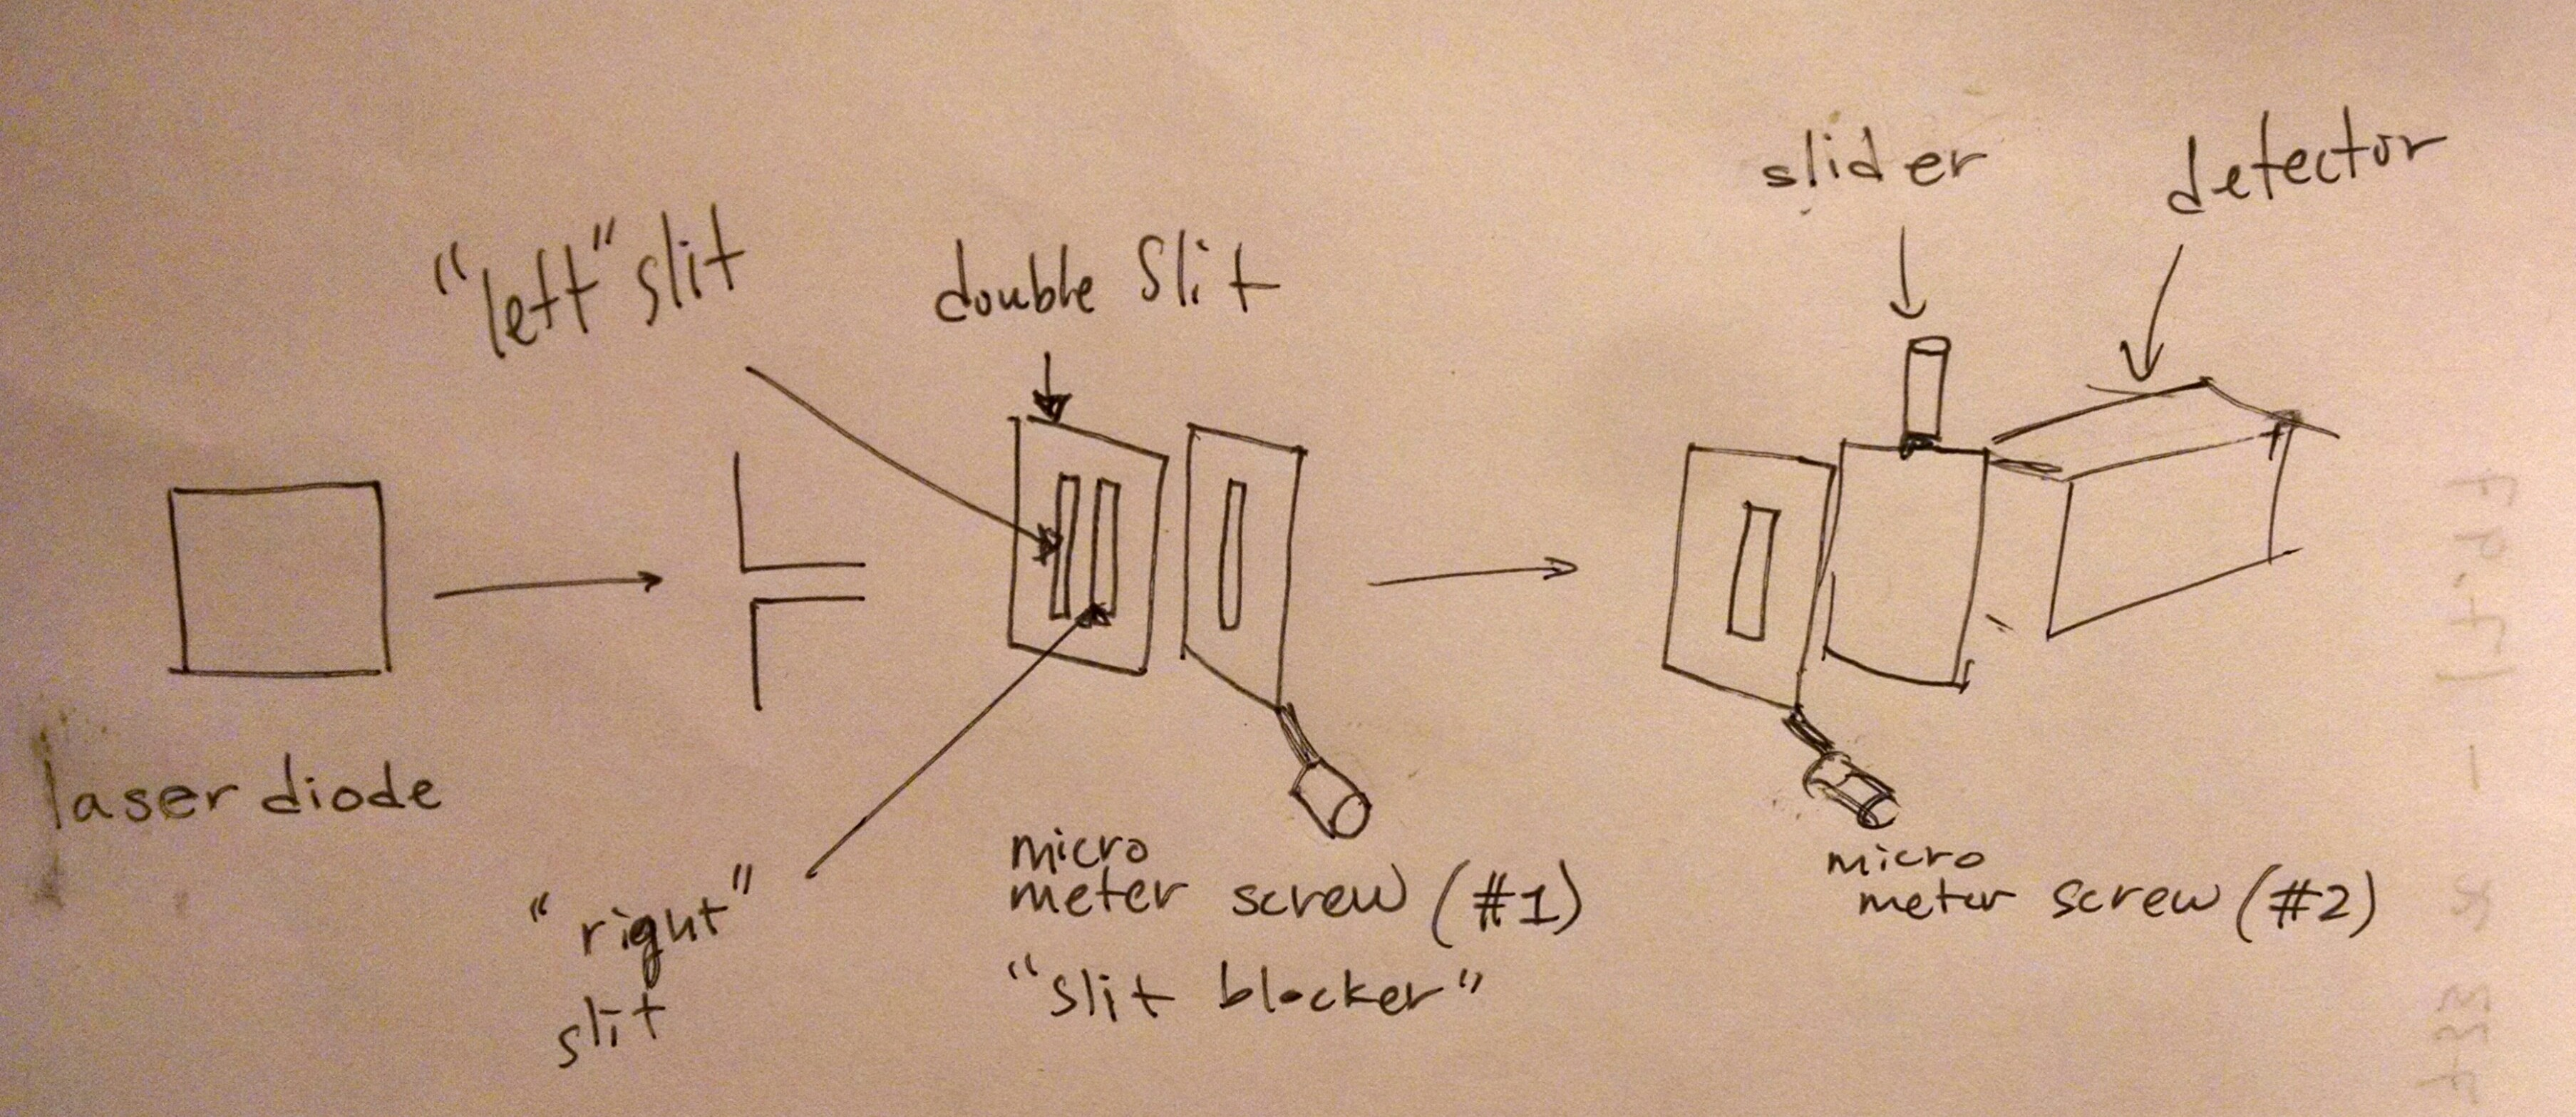
\includegraphics[width=\textwidth]{double_slit_setup.jpg}
    \label{fig:double_slit_setup}
\end{figure}


In order to be able to select the correct slit opening with the box closed. We first had to open the experiment box and find readings on the slit blocker micrometer set screw that corresponded to the having only the left slit open, both slits, and the right slit open. This was done by carefully changing micrometer screw while viewing the outgoing light on a viewing card. We could clearly see the difference in pattern between having one slit open and two slits open because the small line would become twice as thick as with only one slit open. 

Once we had these values we were then able to close the box back up. We set the first micrometer screw to having only the left slit open. We then began the second micrometer set screw at 0.00 mm and took voltage readings every 0.25 mm using a multimeter. We took readings from 0.00 -- 7.00 mm. Beyond the 7.00 mm point there was no change in voltage. Also, we started at 0.00 mm because the micrometer screw does not have negative readings. We repeated the same process for both slits open and only the right slit open. We then generated a plot for each slit opening of the second micrometer screw setting vs. voltage. 

In the second part of the experiment we followed a similar scheme however, we used a photon counter to find intensity. Instead of using the laser we used the light bulb on setting of 6. We had to open up the box to make sure that it was aligned properly. If it was aimed too high or too low the light from the bulb wouldn't make it through the double slit. That would be bad because then we wouldn't be able to get any data, or perhaps poor data. 

We needed to get a baseline voltage for the photon multiplier. If the voltage was too low then the photon counter wouldn't count. If the Voltage was too high we wouldn't be able to see a change. So, we set the second micrometer screw to the central peak of intensity. This meant that the photon counter reading was at a maximum.  Which we found to be around 4.00 mm in the first part of the experiment. Once the micro meter screw was set to the central maximum we started varying the voltage on the photon multiplier. We began at 300 V and increased every 10 V and went up to 650 V(as instructed). We read off the count of photons at each step. We then took the logarithm of the photon count and made a plot of voltage versus logarithm of photon count. This showed that the photon count would level off at a certain voltage. This voltage was chosen to be 460 V. 

Once the voltage was found we then set the first micrometer screw to allow light only through the left slit. We then began the second micrometer screw at 0.00 mm again. We recorded the photon counts every 0.25 mm up to 7.00 mm. This allowed us to make a plot of micrometer screw versus photon count. The same procedure was followed for the double slit, and the right slit as well. 


\section*{Data and Analysis}

In our first experiment we selected a slit setting with the first micrometer screw. We used the settings that we found with the box open. The left setting was at 3.54 mm. Both slits open was at a setting of 4.36 mm on the first micro screw. The right slit was open at 5.26 mm on the micro screw. The slider for the photon multiplier was closed at all times. The voltages were read off from a multimeter hooked up to the end of the box. We decided to increment the second micro screw by 0.25 mm. This decision was only motivated by picking a convenient increment. We added further points if we felt the fidelity of data was not sufficient to fit a curve. The need for more data was implemented for the double slit experiment because originally our data was not as smooth as we liked. We wanted a smooth curve because it then made it easier to see the interference in the graph. The data we collected is in table \ref{voltage_table}

\begin{table}[!htb]
\centering
\caption{Voltage data recorded for three different slit openings. }
\label{voltage_table}
\begin{tabular}{|l|l|l|l|}
\hline
Micro Screw Setting (mm) & Left Slit Open(mV) & Both Slits Open (mV) & Right Slit Open(mV) \\ \hline
0.00                    & 58.6               & 106.1                & 11.7                \\ \hline
0.25                    & 88.1               & 61.4                 & 20.7                \\ \hline
0.50                    & 117.1              & 62.3                 & 34.4                \\ \hline
0.75                    & 148.4              & 310.1                & 51.2                \\ \hline
1                       & 178.7              & 385                  & 72.2                \\ \hline
1.25                    & 204.2              & 75.3                 & 96.1                \\ \hline
1.5                     & 225.8              & 193.3                & 121.9               \\ \hline
1.65                    & --                 & 541                  & --                  \\ \hline
1.75                    & 244.4              & 728                  & 147.7               \\ \hline
2                       & 256.1              & 529                  & 171.6               \\ \hline
2.25                    & 259.7              & 21.1                 & 193.2               \\ \hline
2.5                     & 253.8              & 443                  & 210.6               \\ \hline
2.75                    & 242.6              & 913                  & 222.3               \\ \hline
3                       & 225.2              & 373                  & 228.3               \\ \hline
3.25                    & 205                & 24.3                 & 228.7               \\ \hline
3.35                    & --                 & 175.5                & --                  \\ \hline
3.5                     & 179.6              & 538                  & 222.7               \\ \hline
3.75                    & 151.7              & 667                  & 210.5               \\ \hline
3.85                    & --                 & 475                  & --                  \\ \hline
4                       & 123.2              & 139.7                & 192.2               \\ \hline
4.25                    & 97.1               & 72.7                 & 171.5               \\ \hline
4.35                    & --                 & 200.7                & --                  \\ \hline
4.5                     & 72.7               & 363.1                & 147.6               \\ \hline
4.75                    & 52.9               & 271.6                & 124.7               \\ \hline
5                       & 35.2               & 38.9                 & 101.4               \\ \hline
5.25                    & 22.0               & 67.1                 & 80.4                \\ \hline
5.5                     & 13.0               & 115.4                & 60                  \\ \hline
5.75                    & 10.5               & 54.9                 & 43.5                \\ \hline
6                       &                    & 22.8                 & 29.3                \\ \hline
6.25                    &                    & 18.5                 & 18                  \\ \hline
6.5                     &                    & 10.4                 & 11.1                \\ \hline
6.75                    &                    & 11.2                 & 10.3                \\ \hline
7.00                    &                    & 12.2                 & 10.1                \\ \hline
\end{tabular}
\end{table}

Once the data was collected we created a plot using Microsoft Excel. We then interpolated through the points using the built in Excel program. The plots all the three settings are below. 


\begin{figure}[!ht]
  \caption{Voltage reading for double slit.}
  \centering
    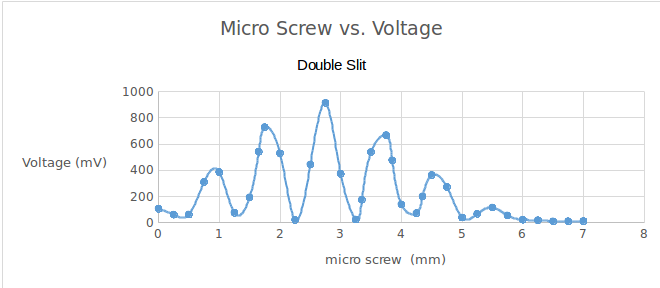
\includegraphics[width=\textwidth]{voltage_double_slit.png}
    \label{fig:voltage double slit}
\end{figure}

\begin{figure}[!ht]
  \caption{Voltage reading for left slit}
  \centering
    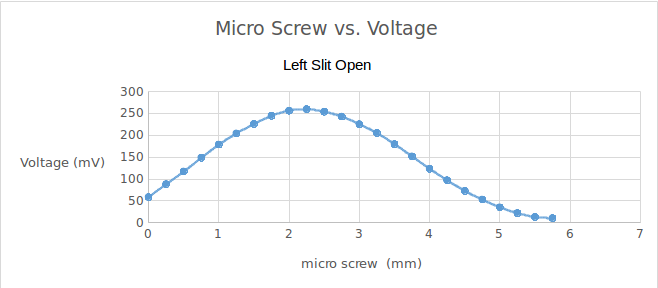
\includegraphics[width=\textwidth]{voltage_left_slit.png}
    \label{fig:voltage left slit}
\end{figure}


\begin{figure}[!ht]
  \caption{Voltage reading for right slit}
  \centering
    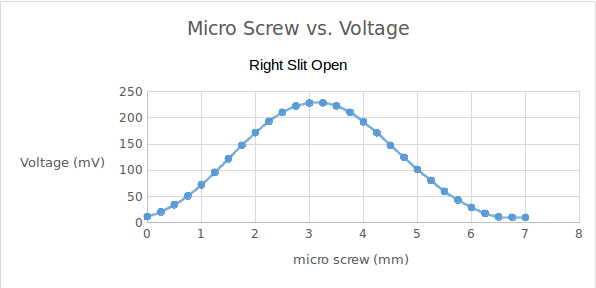
\includegraphics[width=\textwidth]{voltage_right_slit.png}
    \label{fig:voltage right slit}
\end{figure}


In the second part of our experiment we began using the photon multiplier with the light bulb in the box instead of the red laser. Before varying the slits we needed to determine the adequate voltage setting on the photon multiplier. We set the second micrometer screw to the central maximum that we found. We determined the central maximum by setting a voltage and varying the second micrometer screw until we found the highest photon count. 

To verify that the photon counting device was working correctly we turned off the light bulb and saw the photon count decrease. We then turned off the lights in the lab to make sure that no light was getting inside the box. We noted that the photon count did not decrease or increase. 

As instructed in the lab manual we set the light bulb to intensity setting of '6'. We then began the increasing the voltage by 10 V and recording the photon count. This was all done with the photon multiplier slider open and then with the slider closed (i.e. dark count). We chose to increment by 10 V because it seemed like a small enough step size to get a good data. We recorded up to 650 V because that is how high were instructed to go. We then took the logarithm (that is a base 10 $\log$) of each photon count. We did this because we were instructed in the lab manual to create a semi-log graph of the data. Which was done using Libre Office scatter plot methods. Using the software we then interpolated through the points to clearly see that eventually increasing the voltage doesn't increase the photon count as much. The data can be seen here. Where we get an error("Err:502") because the logarithm of zero does not evaluate. The data for this part can be found in table \ref{log_photon_count]}. (Please note: \LaTeX won't put place the table directly below this paragraph because it is too large and woldn't fit on the page.)
\begin{table}[!htb]
\centering
\caption{Data by varying photon multiplier voltage with the slit open and closed. }
\label{log_photon_count]}
\begin{tabular}{|l|p{1.25cm}|p{1.25cm}|l|l|}
\hline
Voltage(V) & Max Count (photon/sec) & Dark Count (photon/sec) & log(max photon count) & log(dark photon count) \\ \hline
300        & 0                             & 0                              & Err:502               & Err:502                \\ \hline
310        & 0                             & 0                              & Err:502               & Err:502                \\ \hline
320        & 0                             & 0                              & Err:502               & Err:502                \\ \hline
330        & 0                             & 0                              & Err:502               & Err:502                \\ \hline
340        & 0                             & 0                              & Err:502               & Err:502                \\ \hline
350        & 1                             & 0                              & 0                     & Err:502                \\ \hline
360        & 6                             & 1                              & 0.7781512504          & 0                      \\ \hline
370        & 20                            & 1                              & 1.3010299957          & 0                      \\ \hline
380        & 50                            & 2                              & 1.6989700043          & 0.3010299957           \\ \hline
390        & 75                            & 4                              & 1.8750612634          & 0.6020599913           \\ \hline
400        & 105                           & 4                              & 2.0211892991          & 0.6020599913           \\ \hline
410        & 130                           & 7                              & 2.1139433523          & 0.84509804             \\ \hline
420        & 175                           & 8                              & 2.2430380487          & 0.903089987            \\ \hline
430        & 180                           & 12                             & 2.2552725051          & 1.079181246            \\ \hline
440        & 191                           & 14                             & 2.2810333672          & 1.1461280357           \\ \hline
450        & 211                           & 18                             & 2.3242824553          & 1.2552725051           \\ \hline
460        & 230                           & 22                             & 2.361727836           & 1.3424226808           \\ \hline
470        & 232                           & 24                             & 2.3654879849          & 1.3802112417           \\ \hline
480        & 237                           & 30                             & 2.374748346           & 1.4771212547           \\ \hline
490        & 249                           & 32                             & 2.3961993471          & 1.5051499783           \\ \hline
500        & 261                           & 46                             & 2.4166405073          & 1.6627578317           \\ \hline
510        & 270                           & 56                             & 2.4313637642          & 1.748188027            \\ \hline
520        & 287                           & 68                             & 2.4578818967          & 1.8325089127           \\ \hline
530        & 293                           & 76                             & 2.4668676204          & 1.8808135923           \\ \hline
540        & 307                           & 79                             & 2.4871383755          & 1.8976270913           \\ \hline
550        & 323                           & 101                            & 2.5092025223          & 2.0043213738           \\ \hline
560        & 326                           & 110                            & 2.5132176001          & 2.0413926852           \\ \hline
570        & 369                           & 130                            & 2.5670263662          & 2.1139433523           \\ \hline
580        & 372                           & 154                            & 2.5705429399          & 2.1875207208           \\ \hline
590        & 409                           & 196                            & 2.611723308           & 2.2922560714           \\ \hline
600        & 454                           & 228                            & 2.6570558529          & 2.357934847            \\ \hline
610        & 556                           & 288                            & 2.7450747916          & 2.4593924878           \\ \hline
620        & 720                           & 340                            & 2.8573324964          & 2.531478917            \\ \hline
630        & 1026                          & 423                            & 3.0111473608          & 2.6263403674           \\ \hline
640        & 1320                          & 509                            & 3.1205739312          & 2.7067177823           \\ \hline
650        & 1376                          & 588                            & 3.1386184339          & 2.7693773261           \\ \hline
\end{tabular}
\end{table}

Once this data was taken we then plotted the values. We can see that the dark count or with the slider closed increases linearly. This is because there is no incoming light. This means that it is increasing strictly because of the increase in voltage of the photon multiplier since that is the only parameter we're changing. By inspection we found that at 460 V the change in voltage does not increase the photon count. We would use 460 V in the next part of the experiment. 

\begin{figure}[!ht]
  \caption{Voltage baseline}
  \centering
    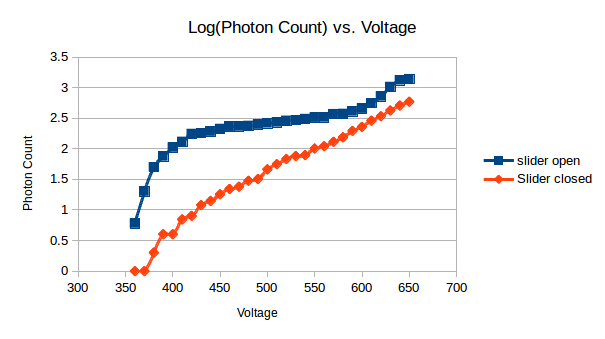
\includegraphics[width=\textwidth]{voltage_baseline.png}
    \label{fig:voltage baseline}
\end{figure}

In the final part of the experiment we set the voltage to 460 V on the photon multiplier. We set the first micrometer screw setting to one of the three settings we found in the first part of the experiment. We began the second micrometer screw at 0.00 mm and incremented by 0.25 mm once again. The micro screw was changed and then we waited about three seconds before taking a reading of photon count. This is because the photon counter would fluctuate for a few seconds before settling to a value. We chose to stop with the left slit at 5.00 mm because we didn't see any change in the voltage. We stopped at 7.00 mm because it seemed that the micro screw wouldn't go further. The data that we collected can be seen in table \ref{photon_count_slits}

\begin{table}[ht!]
\centering
\caption{Photon counts for three different settings. The voltage was set to 460V.}
\label{photon_count_slits}
\begin{tabular}{|l|p{2.5cm}|p{2.5cm}|p{2.5cm}|}
\hline
Micro screw (mm) & Both Slits Open (photon/sec) & Left Slit Open (photon/sec) & Right Slit Open (photon/sec) \\ \hline
0.00             & 45                           & 40                         & 25                          \\ \hline
0.25             & 70                           & 71                         & 22                          \\ \hline
0.50             & 124                          & 89                         & 28                          \\ \hline
0.75             & 100                          & 120                        & 42                          \\ \hline
1.00             & 128                          & 153                        & 62                          \\ \hline
1.25             & 421                          & 187                        & 68                          \\ \hline
1.50             & 238                          & 226                        & 103                         \\ \hline
1.75             & 149                          & 258                        & 132                         \\ \hline
2.00             & 1294                         & 284                        & 160                         \\ \hline
2.25             & 460                          & 290                        & 189                         \\ \hline
2.50             & 125                          & 293                        & 233                         \\ \hline
2.75             & 1599                         & 286                        & 252                         \\ \hline
3.00             & 706                          & 272                        & 264                         \\ \hline
3.25             & 76                           & 218                        & 256                         \\ \hline
3.50             & 917                          & 204                        & 263                         \\ \hline
3.75             & 669                          & 169                        & 244                         \\ \hline
4.00             & 75                           & 132                        & 225                         \\ \hline
4.25             & 324                          & 124                        & 208                         \\ \hline
4.50             & 337                          & 84                         & 169                         \\ \hline
4.75             & 63                           & 55                         & 141                         \\ \hline
5.00             & 128                          & 38                         & 108                         \\ \hline
5.25             & 121                          &                            & 77                          \\ \hline
5.50             & 62                           &                            & 61                          \\ \hline
5.75             & 42                           &                            & 40                          \\ \hline
6.00             & 25                           &                            & 28                          \\ \hline
6.25             & 32                           &                            & 22                          \\ \hline
6.50             & 37                           &                            & 21                          \\ \hline
6.75             & 37                           &                            & 18                          \\ \hline
7.00             & 42                           &                            & 24                          \\ \hline
\end{tabular}
\end{table}


The data in table \ref{photon_count_slits} was used to create a scatter plot. This was done using Microsoft Excel's scatter plot function. We Excel to interpolate through the points. This gave us an understanding of the data where we can clearly see the interference pattern. (It seems better suited to discuss results in the results section.)

\newpage

\vspace*{-20cm}

\begin{figure}[!h]
  \caption{Photon count of double slit}
  \centering
    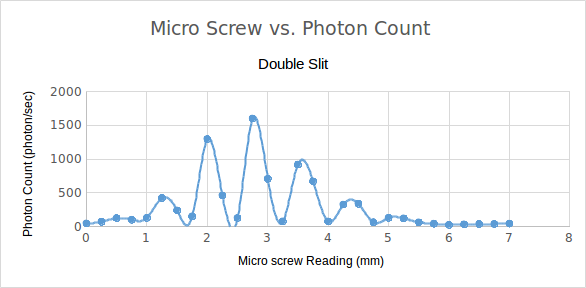
\includegraphics[width=\textwidth]{photon_count_double_slit.png}
    \label{fig:photon_double}
\end{figure}

%\vspace*{100cm}

\begin{figure}[!h]
  \caption{Photon count of left slit}
  \centering
    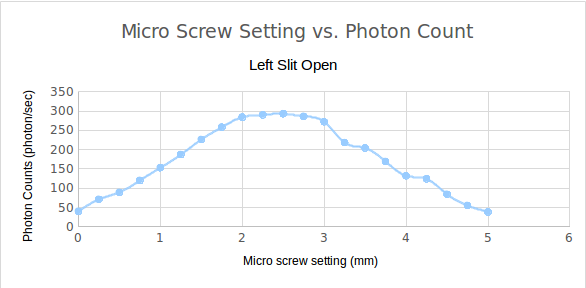
\includegraphics[width=\textwidth]{photon_count_left_slit.png}
\end{figure}

\vspace*{3cm}

\begin{figure}[!h]
  \caption{Photon count of right slit} 
  \centering
    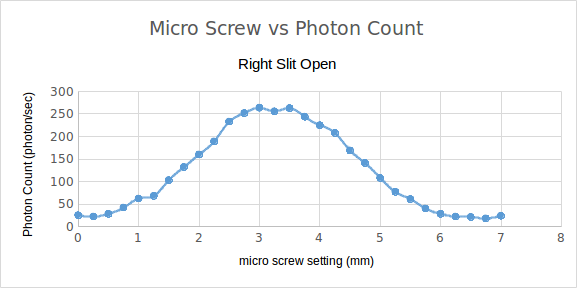
\includegraphics[width=\textwidth]{photon_count_right_slit.png}
\end{figure}




\vspace*{60cm}

\section*{Results and Conclusions}

In this experiment our main result was finding that constructive and destructive interference takes place when both a red laser or light bulb are put through a double slit. The constructive interference leads to an increase of intensity as seen in a peaks of intensity. The destructive interference creates a near zero intensity. Both constructive and destructive interference can be clearly seen in the double slit plots of figure \ref{fig:voltage double slit} and figure \ref{fig:photon_double}. The constructive interference are the peaks of intensity(i.e voltage or photon count) and the destructive interference are the troughs of zero intensity. 

It would seem that interference doesn't take place when the light goes through a single slit in our experiment. Fraunhofers's theory would predict that we should see diffraction in the single slit, and the double slit. However, we did not see a trace of diffraction for our four single slit settings. Perhaps this was because we did not take readings out far enough(with micrometer screw 2). We might also have not seen the diffraction because the the sensitivity is not high enough in our methods. It would seem that theoretically the increase of intensity to the left and right of the main peak is small in comparison to main peak. 

Interestingly we can see that since the peaks and troughs of the double slit experiments are at slightly different locations. This shows that the red laser and the light bulb are indeed at different wavelengths. This is because the different wavelengths will then interfere at different points.  

Also, as instructed, when we were measuring the photon count at the central maximum we were getting readings of around 1400 photons/sec with the double slit. We then switch to the left slit being open. When we did this we saw the photon count drop. We hypothesize that this is because the central peak of the double slit is not at the same spot at the maximum for the left or right slit. The drop in photon count was less than 50\% because the central peak was only shifted to the left. Similarly, if we place the detector slit at a point of complete destructive interference and then switched to a left or right slit we can see an increase in intensity. We hypothesize that this is because the destructive interference doesn't happen with a single slit being open, and it especially doesn't happen at the same point as the double slit. 

In conclusion, we have found without question that light exhibits a wave like nature that can be seen when put through a double slit. 

\end{document}